\chapter{LOCAL MOTOR INVARIANT}
\label{chap:li}

\nomenclature{$G$}{A Lie Group}
\nomenclature{$g_a$}{an elemetn in Lie Group $G$ with parameter $a$}
\nomenclature{$I(x)$}{Invariant Function of $x$}
\ifpdf
    \graphicspath{{LocalInvariant/LocalInvariantFigs/PNG/}{LocalInvariant/LocalInvariantFigs/PDF/}{LocalInvariant/LocalInvariantFigs/}}
\else
    \graphicspath{{LocalInvariant/LocalInvariantFigs/EPS/}{LocalInvariant/LocalInvariantFigs/}}
\fi

\section{Introduction}
Global Motor Invariant Control keeps the qualitative properties of motion primitives.
For animal motion is also of high accuracy.
In this chapter we focus on the control on the quantitative properties of motion.
In our research, we try to limit the computational cost.


The discovery is that motion of natural system will change in a uniform way.
The method we proposed exploring the symmetry properties of dynamics system.
The symmetry property of a dynamic system is called local motor invariant.
The method we propose is based the lie group theory,please refer to book\citep{olver1986applications}
for more details.

\subsection{Group and Symmetry}
For the geometrical viewpoint, ''Symmetry''  means when you transform an shape, the transform one and original one are exactly the same.
For the square examples, rotation it by 90 degree will make it exactly the same with the original one.



\begin{figure}[!htbp]
  \begin{center}
      \includegraphics[width=0.7\textwidth]{Symmetry}
    \caption{Symmetry}
    \label{fig:symmetry}
\end{center}
\end{figure}


All the action that can preserve the symmetry is defined as the set as group $G$.
A group has the following properties.
\begin{itemize}
\item For any $g_a,g_b$ in $G$, \,$g_a*g_b$\, belongs to $G$. (The operation
``$*$'' is closed).

\item For any \,$g_a,g_b,g_c\in G$, \,$(g_a*g_b)*g_c=g_a*(g_b*g_c)$. \,(Associativity of
the operation).

\item There is an element $e\in G$ such that \,$g_a*e=e*g_a=g_a$\, for any
\,$g_a\in G$. (Existence of identity element).

\item For any \,$g_a\in G$\, there exists an element $g_h$ such that
\,$g_a*g_h=g_h*g_a=e$. \,(Existence of inverses).
\end{itemize}

for the shape geoemtry example example $g_1$ is rotate 90 degree clockwise. then $e$ is no rotation.
we also know $g_2=g_1*g_1$ is rotate 90 degree clockwise twice.$g_2$ also preserve the shape.


In algebra sense, ''Symmetry'' means invariant, a shape can implicitly defined by an function $I(x)=0$;
The group transformation is define by $\hat{x}=g_a(x)$
If symmetry is met, we have $I(x)=I(\hat{x})$.
We can say $I(x)$ is an invariant function of group $G$.

We have to note that not only the one shape unchanged by $G$.
In fact ,many shape is invariant, 
In fact, we can pick up and two shape and combination is also an invariant shape. 
and form a space, the invariant space $I(x)$.


\begin{figure}[!htbp]
  \begin{center}
    \leavevmode
    \ifpdf
      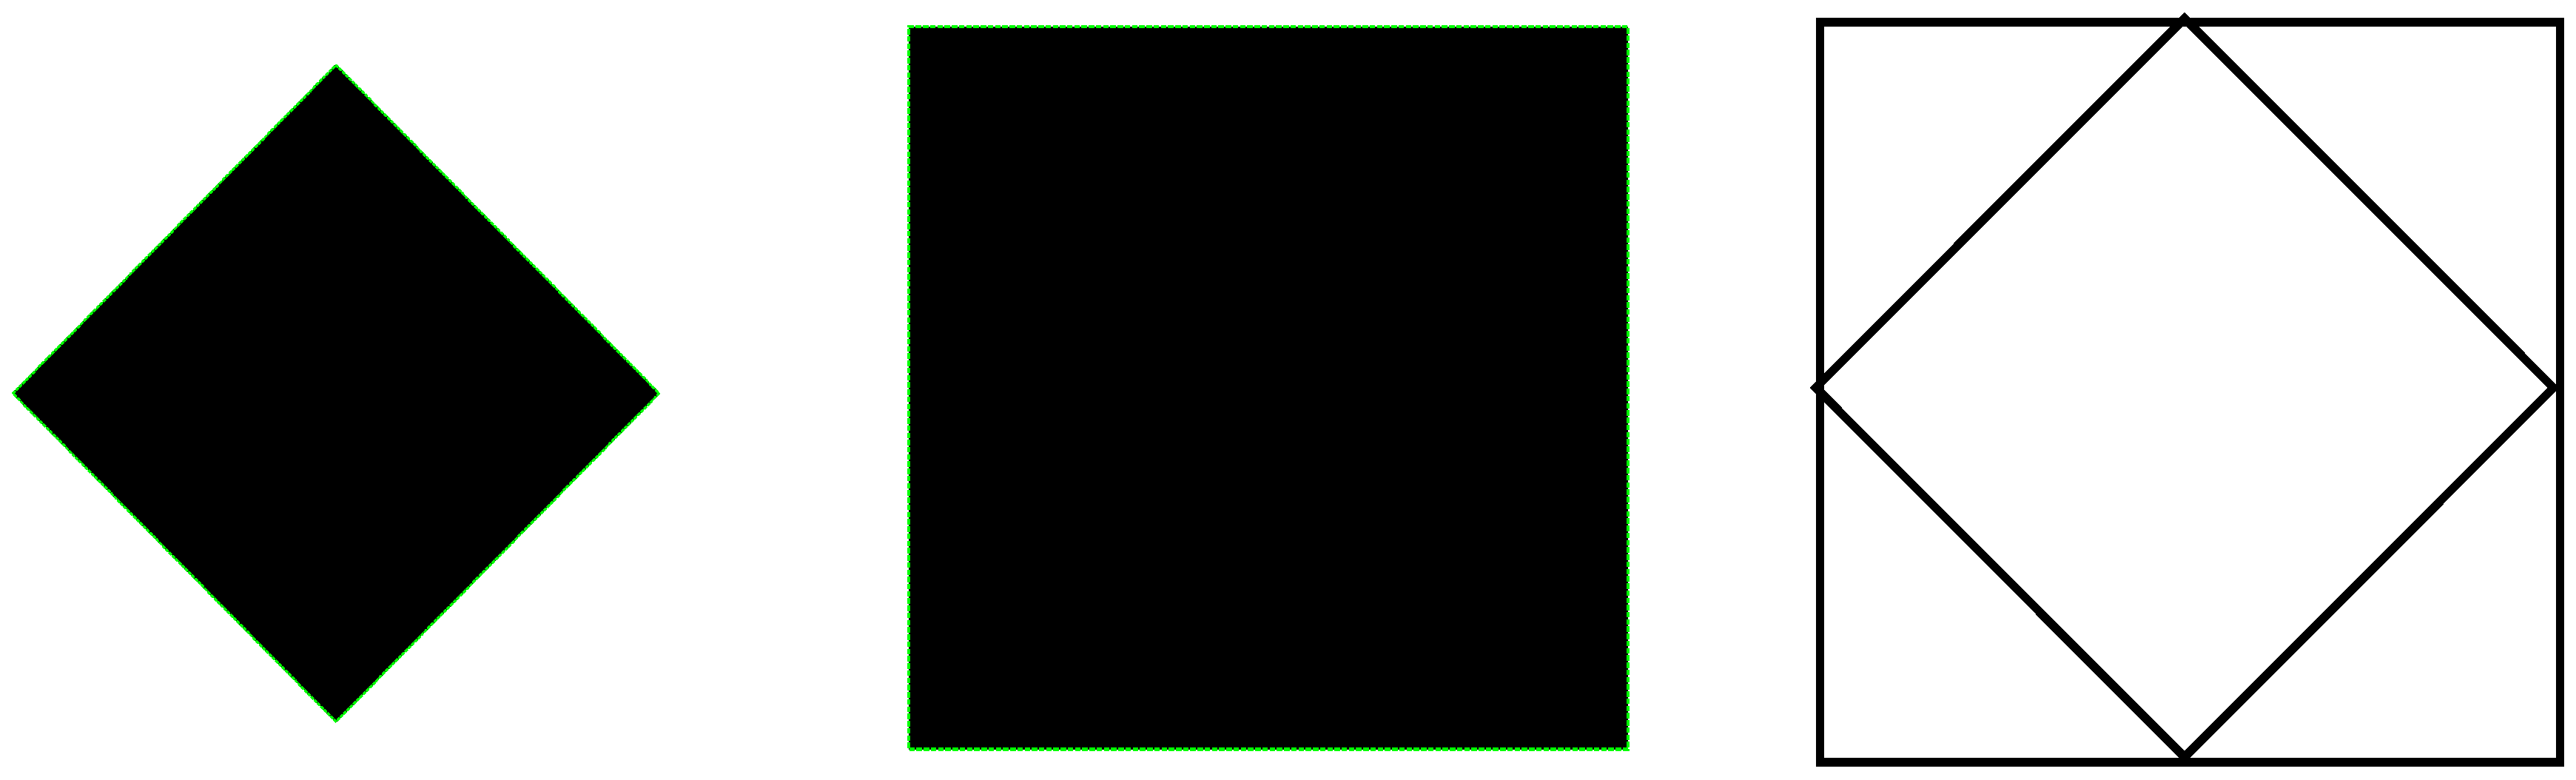
\includegraphics[height=6in]{SymmetrySpace}
    \else
      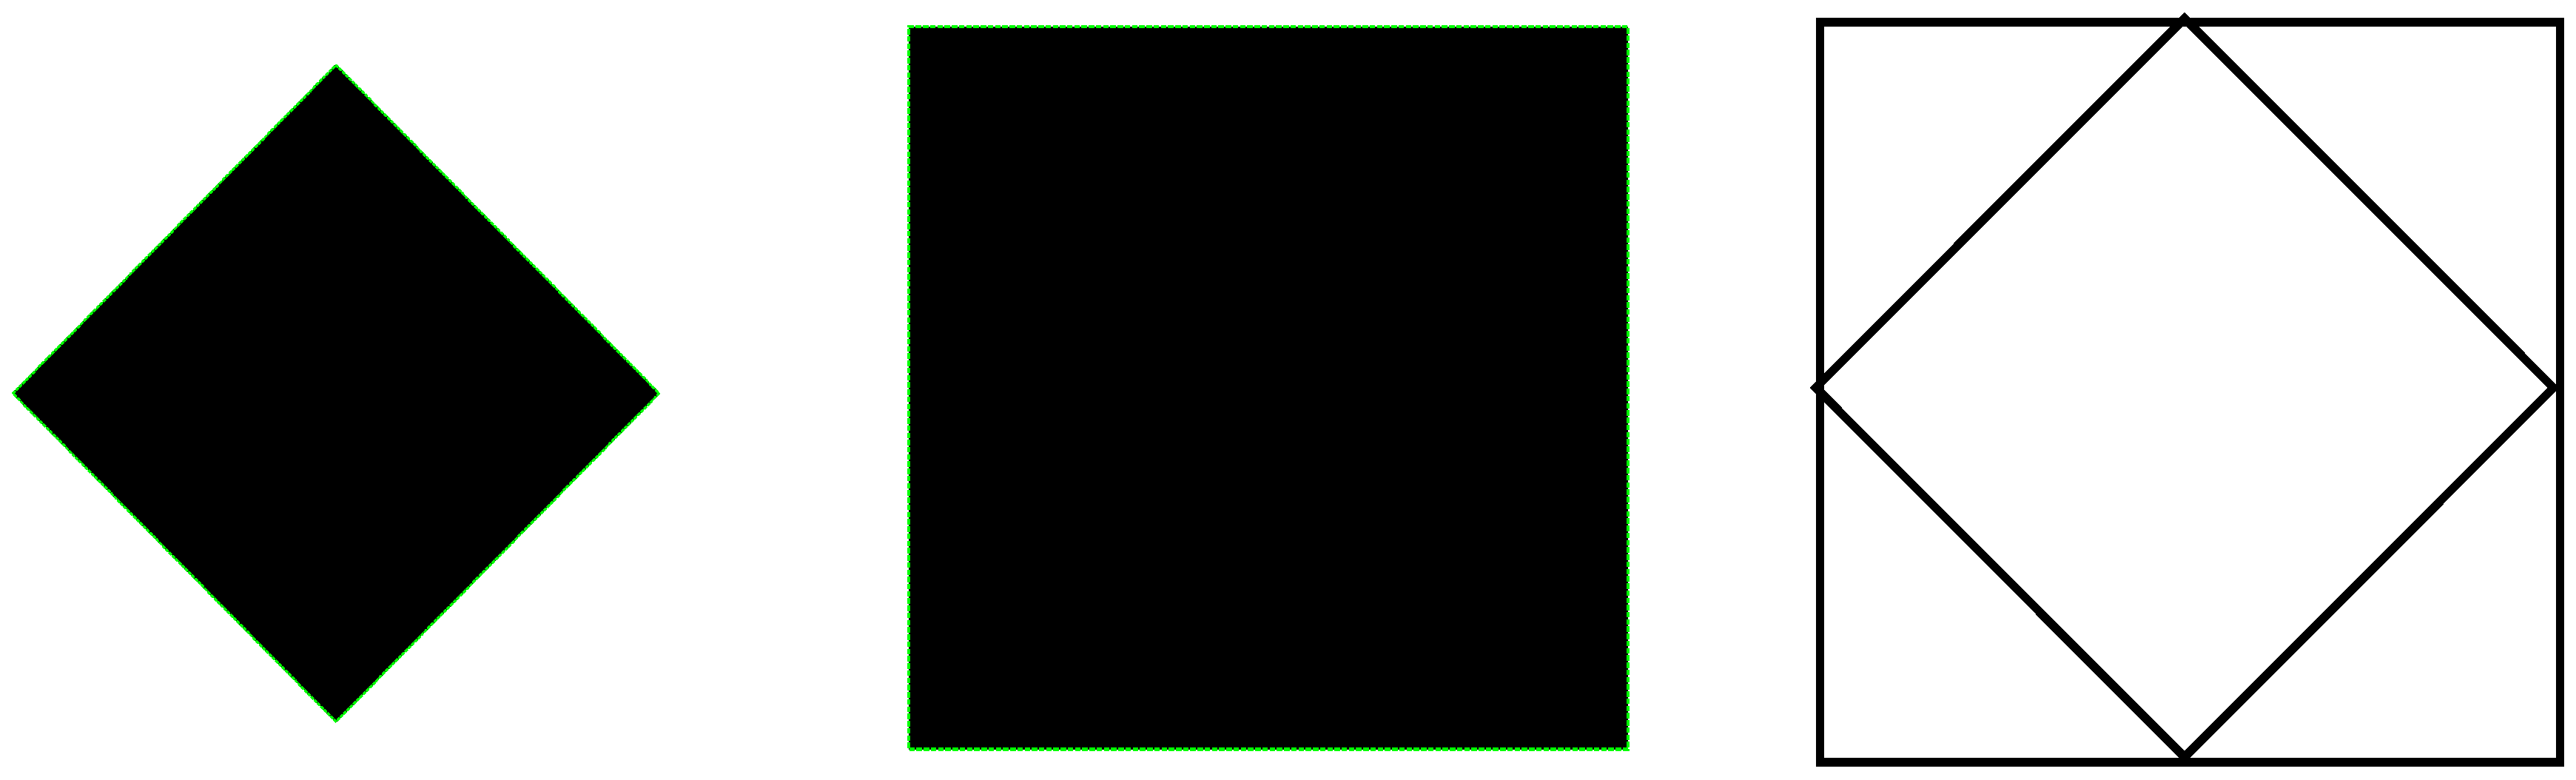
\includegraphics[width=0.7\textwidth]{SymmetrySpace}
    \fi
    \caption{Symmetry Space}
    \label{fig:symmetry Space}
\end{center}
\end{figure}





\subsection{Lie Group and Symmetry of Dynamic System}
The rotate group is discrete.
if the shape is circle, than the rotation is continues, the continues group is Lie Group.

Lie Group is continues group originates from study of differential equation.
For Physically-based animation,
Motion is usually described by the differential equation (1)
\begin{equation}
	\dot{\state}=F(\state)
\end{equation}
Lie Group $G$ will perserve the differential equation,for $g_a \in G$ 
\[
Tg_a(\dot{\hat{\state}})=F(g_a(\state)
\]
where $Tg_a$ is the corresponding lift action that transform the velocity $\dot{\state}$.
for example, if the $g_a$ is translate transformation, velocity will not be translate, then $Tg_a$ is identy.





Physically possible motion is the solution of the equation.
An important property from one solution $\state(t)$.
with a group action $g_a$, we can get another solution $g_a(\state(t))$
 	
for the mass spring system ~\ref{eq:stateform}
we apply the group action 
\[
\hat{\state}=g_a(\state)=[\alpha q, \alpha \qd ]
\]
then the lift action is
\[
\dot{\hat{\state}}=Tg_a(\state)=[\alpha \qd, \alpha \ddot{q}]
\]



by substitution $\state \mapsto \hat{\state}$, the original system become
\[ 
\dot{\hat{\state}}=
\left[ 
\begin{array}{cc}
0 &1\\
-1 &0 
\end{array}
\right]\hat{\state}
\]
which is 
\begin{equation}
\label{eq:tranmas} 
\alpha \dot{\state}=
\left[ 
\begin{array}{cc}
0 &1\\
-1 &0 
\end{array}
\right]\alpha \state
\end{equation}

equation ~\ref{eq:tranmas} is equivalent to  ~\ref{eq:stateform}
thus if $\state(t)$ is a solution, we get another solution $\hat{\state}(t)$.

such transformation form a group.
we define 
\[
g_{\alpha}*g_{\beta}(\state)=[\alpha \beta q, \alpha \beta \qd]
\]
which also satisfy the differential equation.

and 
\[
g_{\alpha}^{-1}=g_{\frac{1}{\alpha}}
\]
when $\alpha \in R^+$, the group is continues,
thus it is an example of Lie Group.





This provide us an idea about motion synthesis.
Given an original motion $q(t)$, and the corresponding group $G$, a new motion is generated by transformation.
For every group G, we can find an function $I(x)$ unchanged by the group action G, 

$I(\state)$ are called local motion invariant. 
For mechanical system,  $I(x)$ has important physically meaning. 
$I(\state)$ corresponding to the Conservative Law like energy or angular momentum.


\section{Controlled Symmetry}
For motion synthesis, usually the desired motion is ma
For example for motio stability, we want the current state is within the basin of attraction.
If we want to control the final motion style, we want the state is on the limit cycle.

For motion sysnthesis, the problem is given the system, let the original system have the desired symmetry.

 and original motion m is  known, but the corresponding group action $g_a$ is not satisfied by differential equation.
For such situation, control input u  is added, which modify the original equation to allow the designed $G$, this is called Controlled Symmetry.

Most dynamic motion can be modelled as an Lagrange System. 
\[
L=K(\dot(q)-V(q).
\]
And the desired action $G$ must keep the $L$ invariant. 

The original m is defined by the eural langrage equation
\begin{equation}
\frac{d}{dt} \frac{\partial L}{\partial \qd} - \frac{\partial L}{\partial q} = 0
\label{eq:uncontrolled_euler_lagrange}
\end{equation}
The modified system is 
\begin{align}
\frac{d}{dt} \frac{\partial L}{\partial Tg(\qd)} - \frac{\partial L}{\partial g(q)}&=0,\label{eq:liegroup_euler_lagrange}\\
\frac{d}{dt} \frac{\partial L}{\partial \qd} - \frac{\partial L}{\partial q}&=\ulocal. \label{eq:controlled_euler_lagrange}
\end{align}


(5) and (6) are the equivalent equation, by comparing  equation (5) and (6), we can get $u$
Some Specific example of Symmetry and Control.
In the following discussion, suppose all the group element $g$ are paramerizate by the parameter $\alpha$.

\subsection*{ Offset Action}
we move the posture of the system 
\[
q \mapsto q+\alpha
\]
then the offset transformation is
\[
\goff(\state) = [q+\alpha,\qd]
\]


\begin{equation}
\ulocal(q) = \frac{\partial}{\partial q} \left(V(\goff(q)) - V(q)\right).
\end{equation}

if we formulate the controlled mass spring system in the followign way~\ref{eq:controlmass}
\begin{equation}
\label{eq:controlmass}
\ddot{q}+q=\ulocal
\end{equation}

for the mass spring system.
\[
\ulocal(q)=\alpha
\]

\begin{figure}[!htbp]
  \begin{center}
      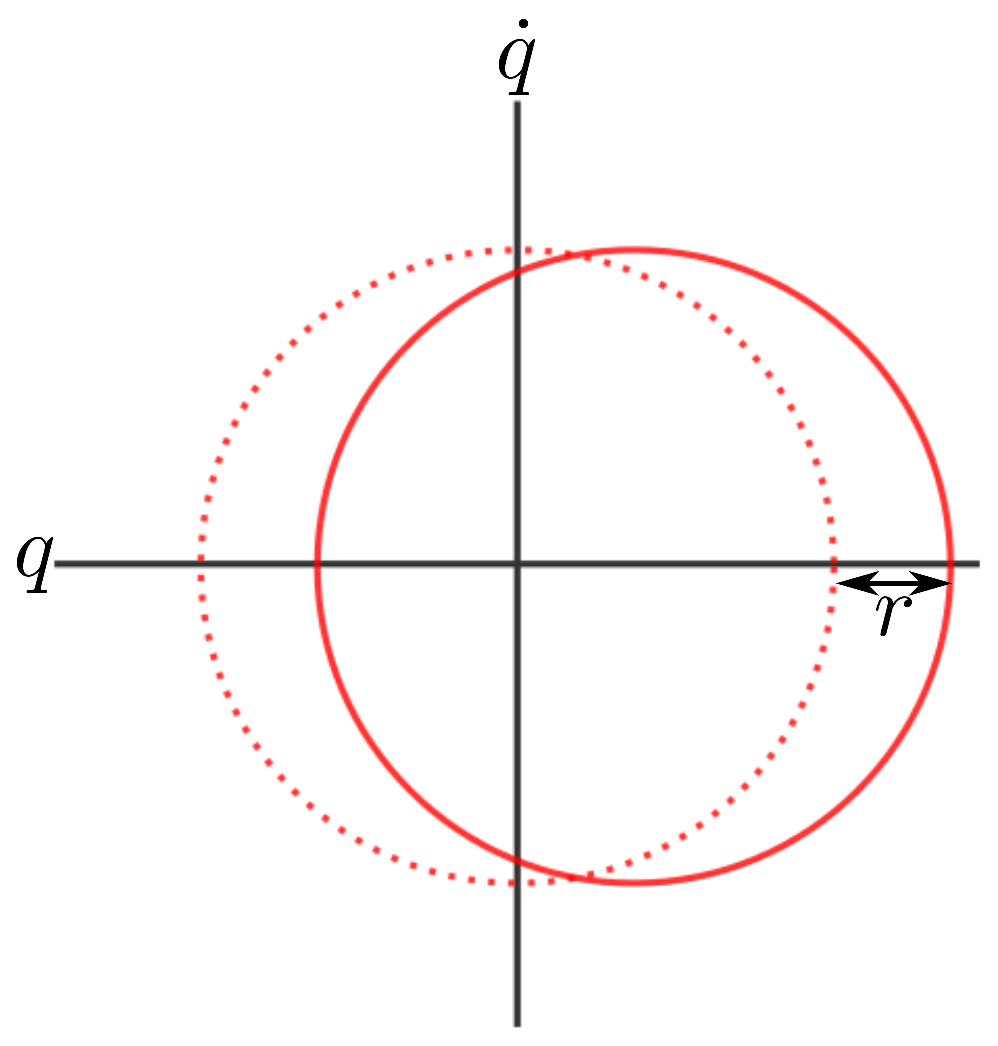
\includegraphics[width=0.7\textwidth]{g_off}
    \caption{Offset Action}
    \label{fig:goff}
\end{center}
\end{figure}
on phase space, if $q$ is the horizontal axis, and $\dot{q}$ is the vertical axis, this has the effect of moving the phase plot horizontally.

\subsection*{Time Scalling}

%g_st(q,dot{q})=(q,st*dot{q})
if we scale the time paramter
\[
t \mapsto \frac{t}{\alpha}
\]

we have
\[
\gts(\state)=[q,\alpha \qd]
\]
\[
T\gts(\dot{\state})=[\alpha \qd,\alpha^2 \ddot{q}]
\]
Then the local control is 
\begin{equation}
\ulocal(q) = (\alpha^2 - 1) \frac{\partial V(q)}{\partial q}.
\end{equation}

for the mass spring system in
\[
\ulocal=(\alpha^2-1)q
\] 

\begin{figure}[!htbp]
  \begin{center}
    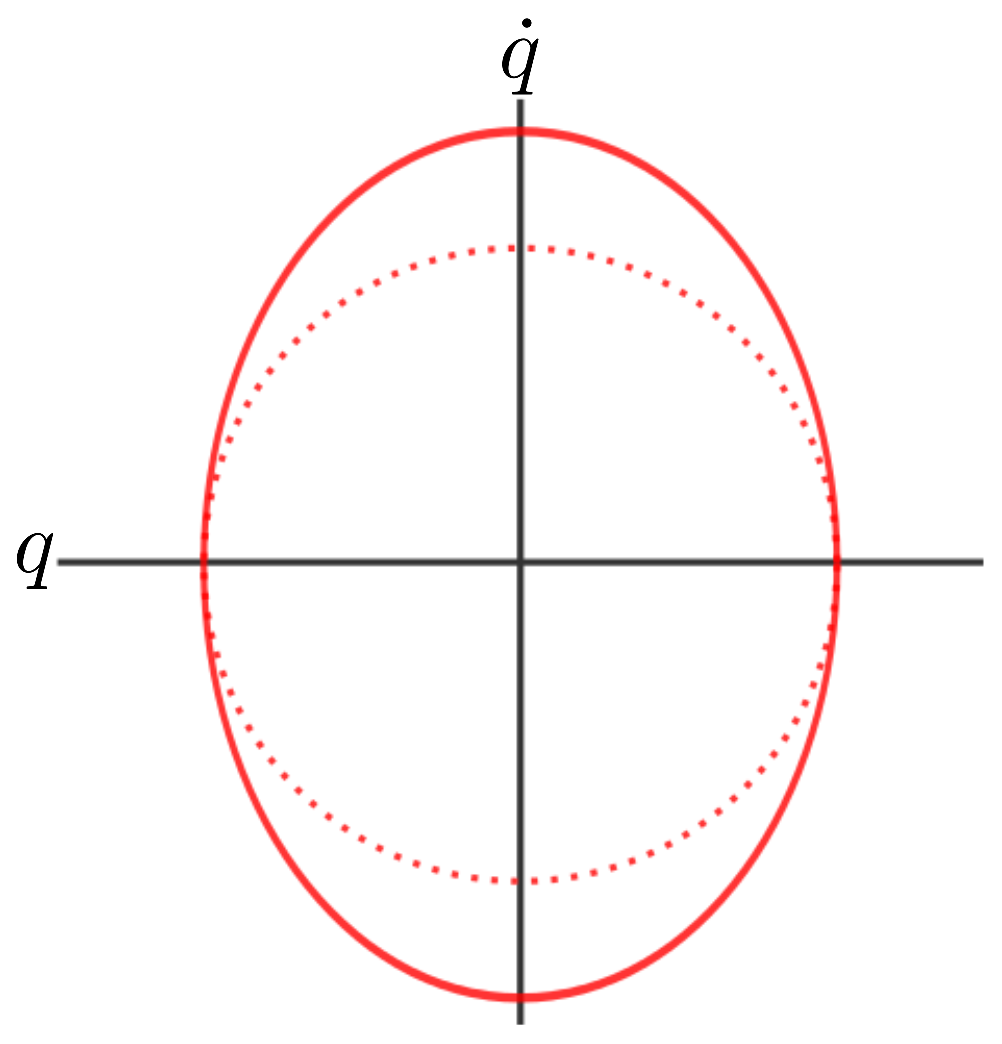
\includegraphics[width=0.7\textwidth]{g_ts}
	 \caption{Time Scaling Action}
    \label{fig:gts}
\end{center}
\end{figure}
on phase space, this has the effect strength the phase plot in the vertical direction

\subsection*{Energy Scaling}
For some system moving the the conservtive field.
The energy is preserved and different motion present different level of energy.
For such system, we have the the energy $E(\state)=K+V$, where $K$ is the kinematic energy,
$V$ is the potential enegy.
\[
E(\hat{\state})=\alpha^2 E(x)
\]
if the the mass of system is constant.
\[
\gen(\state)=(f(\alpha) q,\alpha \dot{q}).
\]
where $f(\alpha)$ is a funtion of $\alpha$, which depends on the shape of potential field.
$\ulocal$ can be developed by applying the pos scaling and time scaling in a combined manner.



for the mass spring system , $E=\frac{1}{2}(q^2+\qd^2)$,$f(\alpha)=\alpha$, and because the energy scaling is kept by the original system, we have
\[
\ulocal=0
\]
On phase plot, this has the effect enlarge the phase portrait.

\begin{figure}[!htbp]
  \begin{center}
      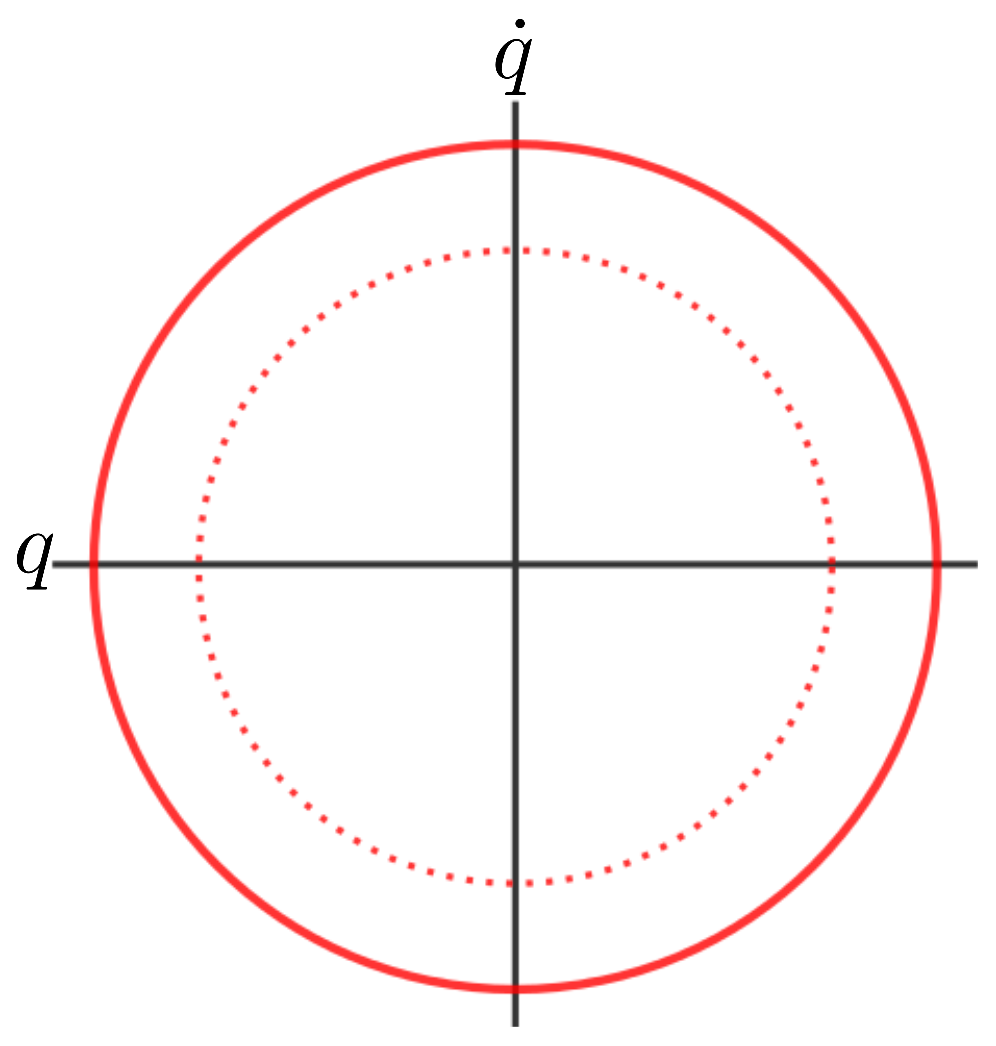
\includegraphics[width=0.7\textwidth]{g_en}
    \caption{Energe Scaling Action}
    \label{fig:gen}
\end{center}
\end{figure}


\subsection*{Time Offset}
we can also offset the time $t$
\[
t \mapsto t+\alpha
\]
\[
\gtd(\state(t))=[q(t+\alpha),\qd(t+\alpha)]
\]
For dynamic system, this seems obvious. And no control is need for such symmetry.
For system with limit circle, this $\gtd$ has a special effects like phase modification.

On phase plot, this has the effect rotate on the limit circle about an angle.
\begin{figure}[!htbp]
  \begin{center}
      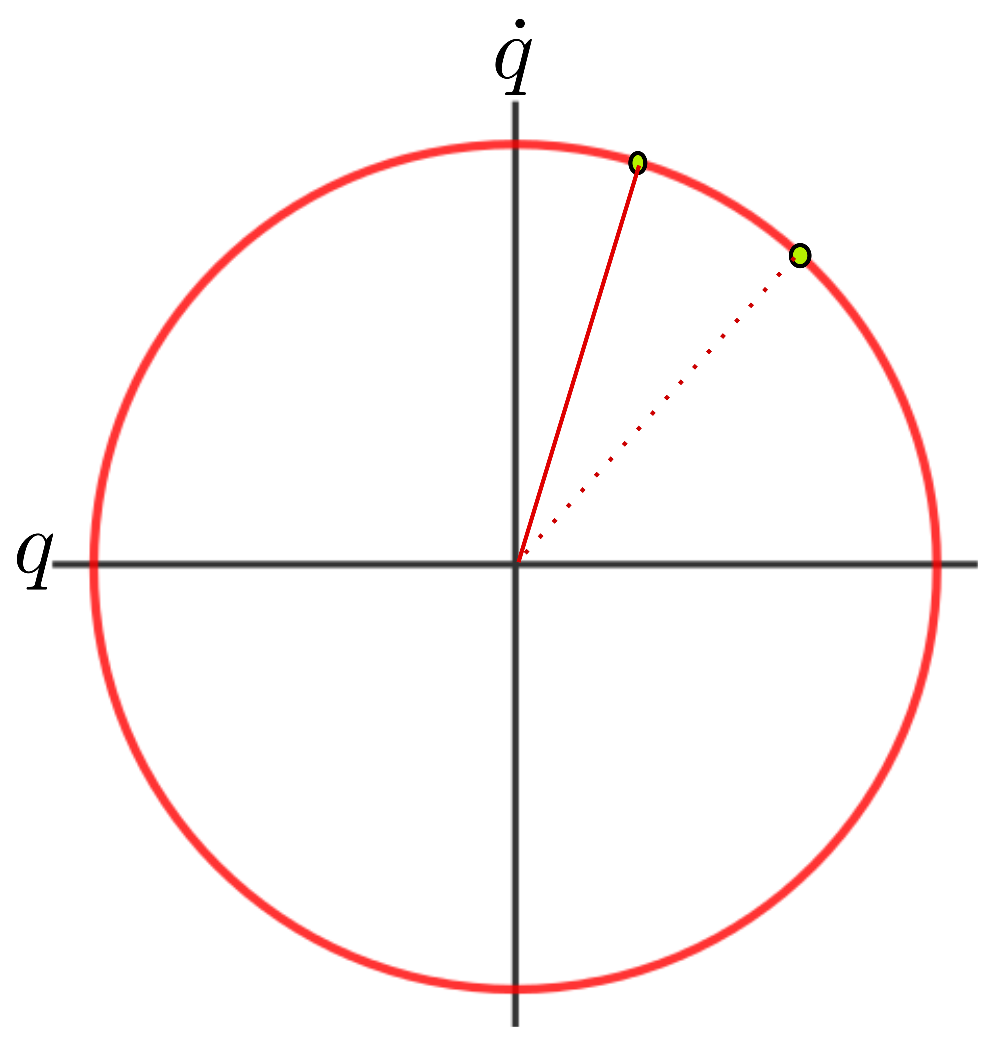
\includegraphics[width=0.7\textwidth]{g_toff}
    \caption{Offset Action}
    \label{fig:gtoff}
\end{center}
\end{figure}





\section{Example:Bouncing Ball dropt frome Different Height}
Even it is a hybrid system,
The bouncing ball system has a energy scaling symmetry.

the ennegy function 
\[
E=g_{ravity}h+\frac{1}{2}m\qd^2
\]
so the 
\[
f(\alpha)=\alpha^2
\]

then the energy scaling action is
\[
\gen(\state)=[\alpha^2 q, \alpha \qd]
\]

given the motion of droping at 5 are shown in Figure~\ref{bouncing5}.


\begin{figure}[!htbp]
  \begin{center}
      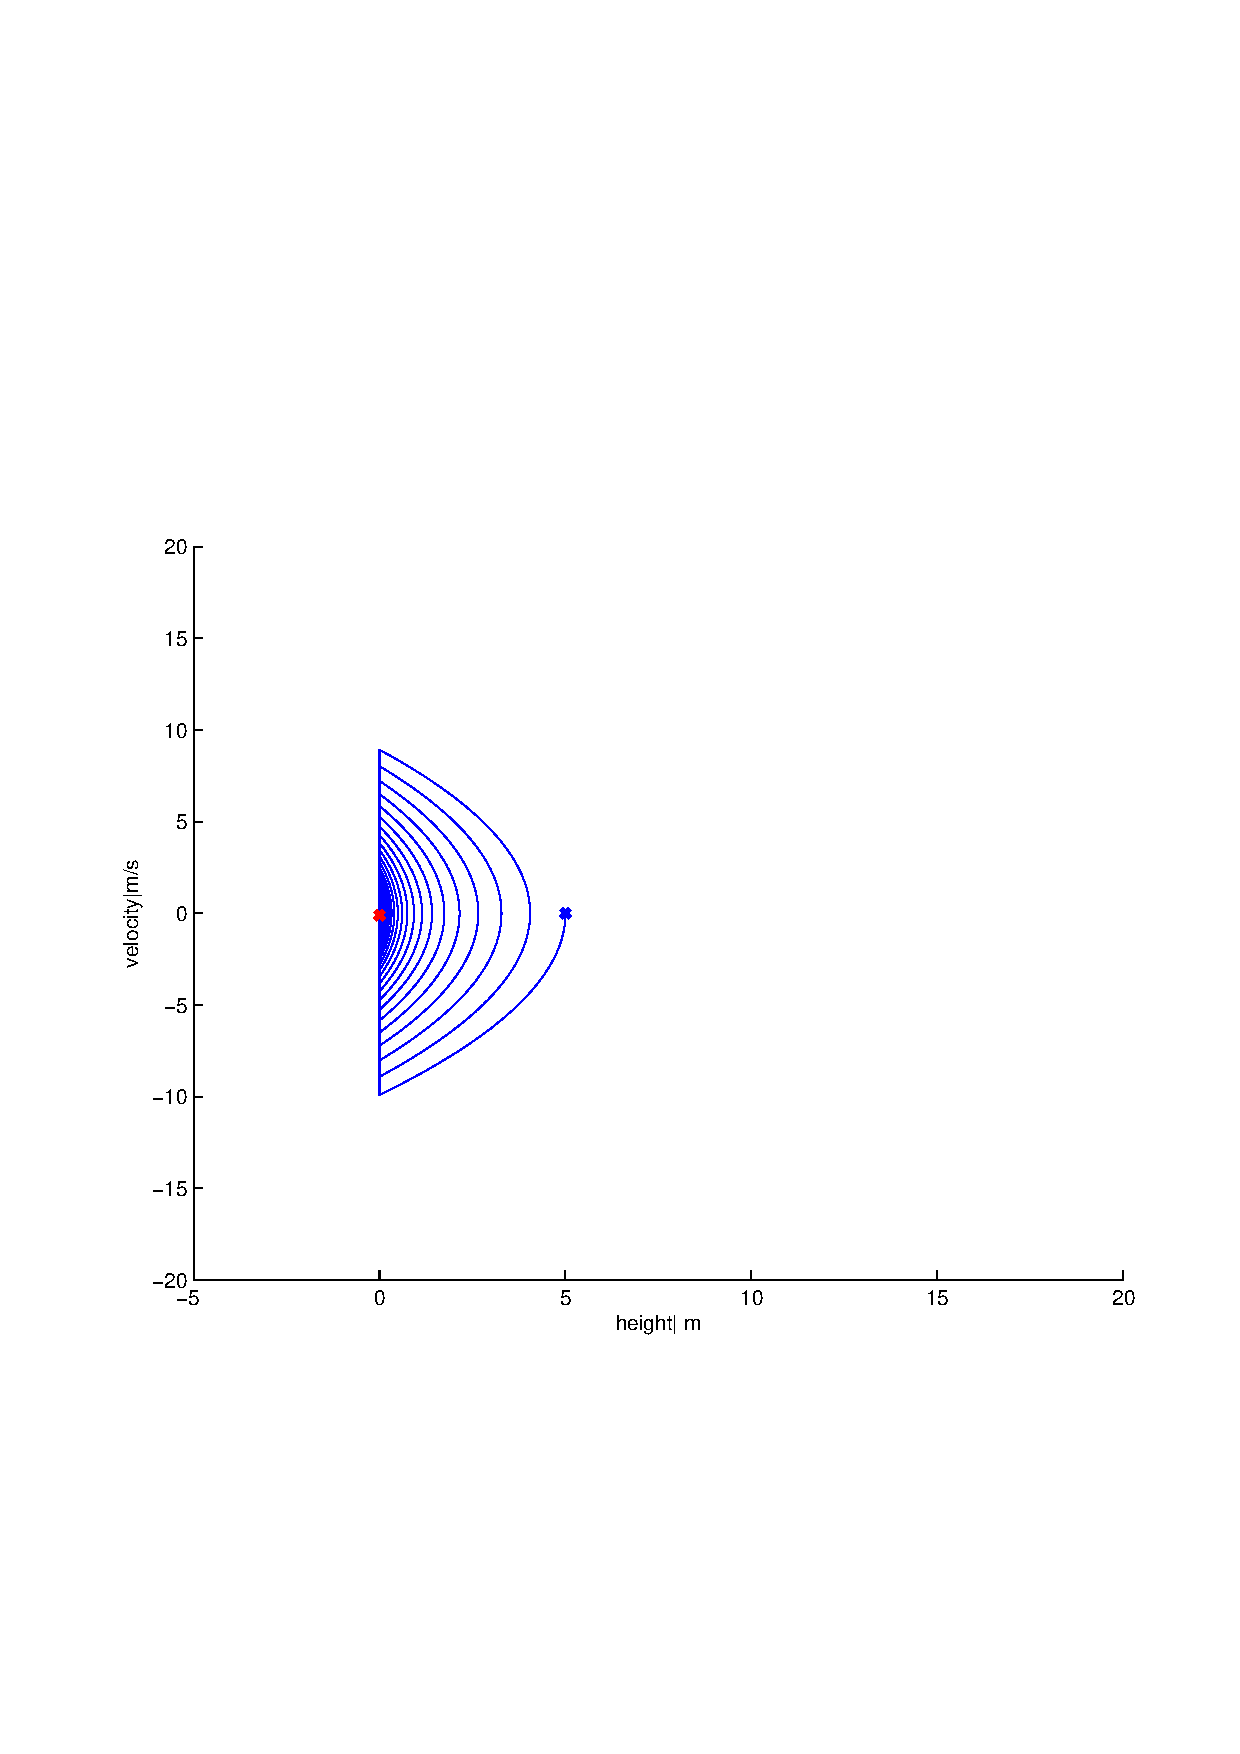
\includegraphics[width=0.7\textwidth]{BouncingBallPhasePlotuncontrolledDropAt5}
    \caption{Drop at 5}
    \label{fig:bouncing5}
\end{center}
\end{figure}

if $\alpha=\sqrt{2}$, we get the bouncing motion drop at height 10, as show in figure ~~\ref{bouncing5}
\begin{figure}[!htbp]
  \begin{center}
      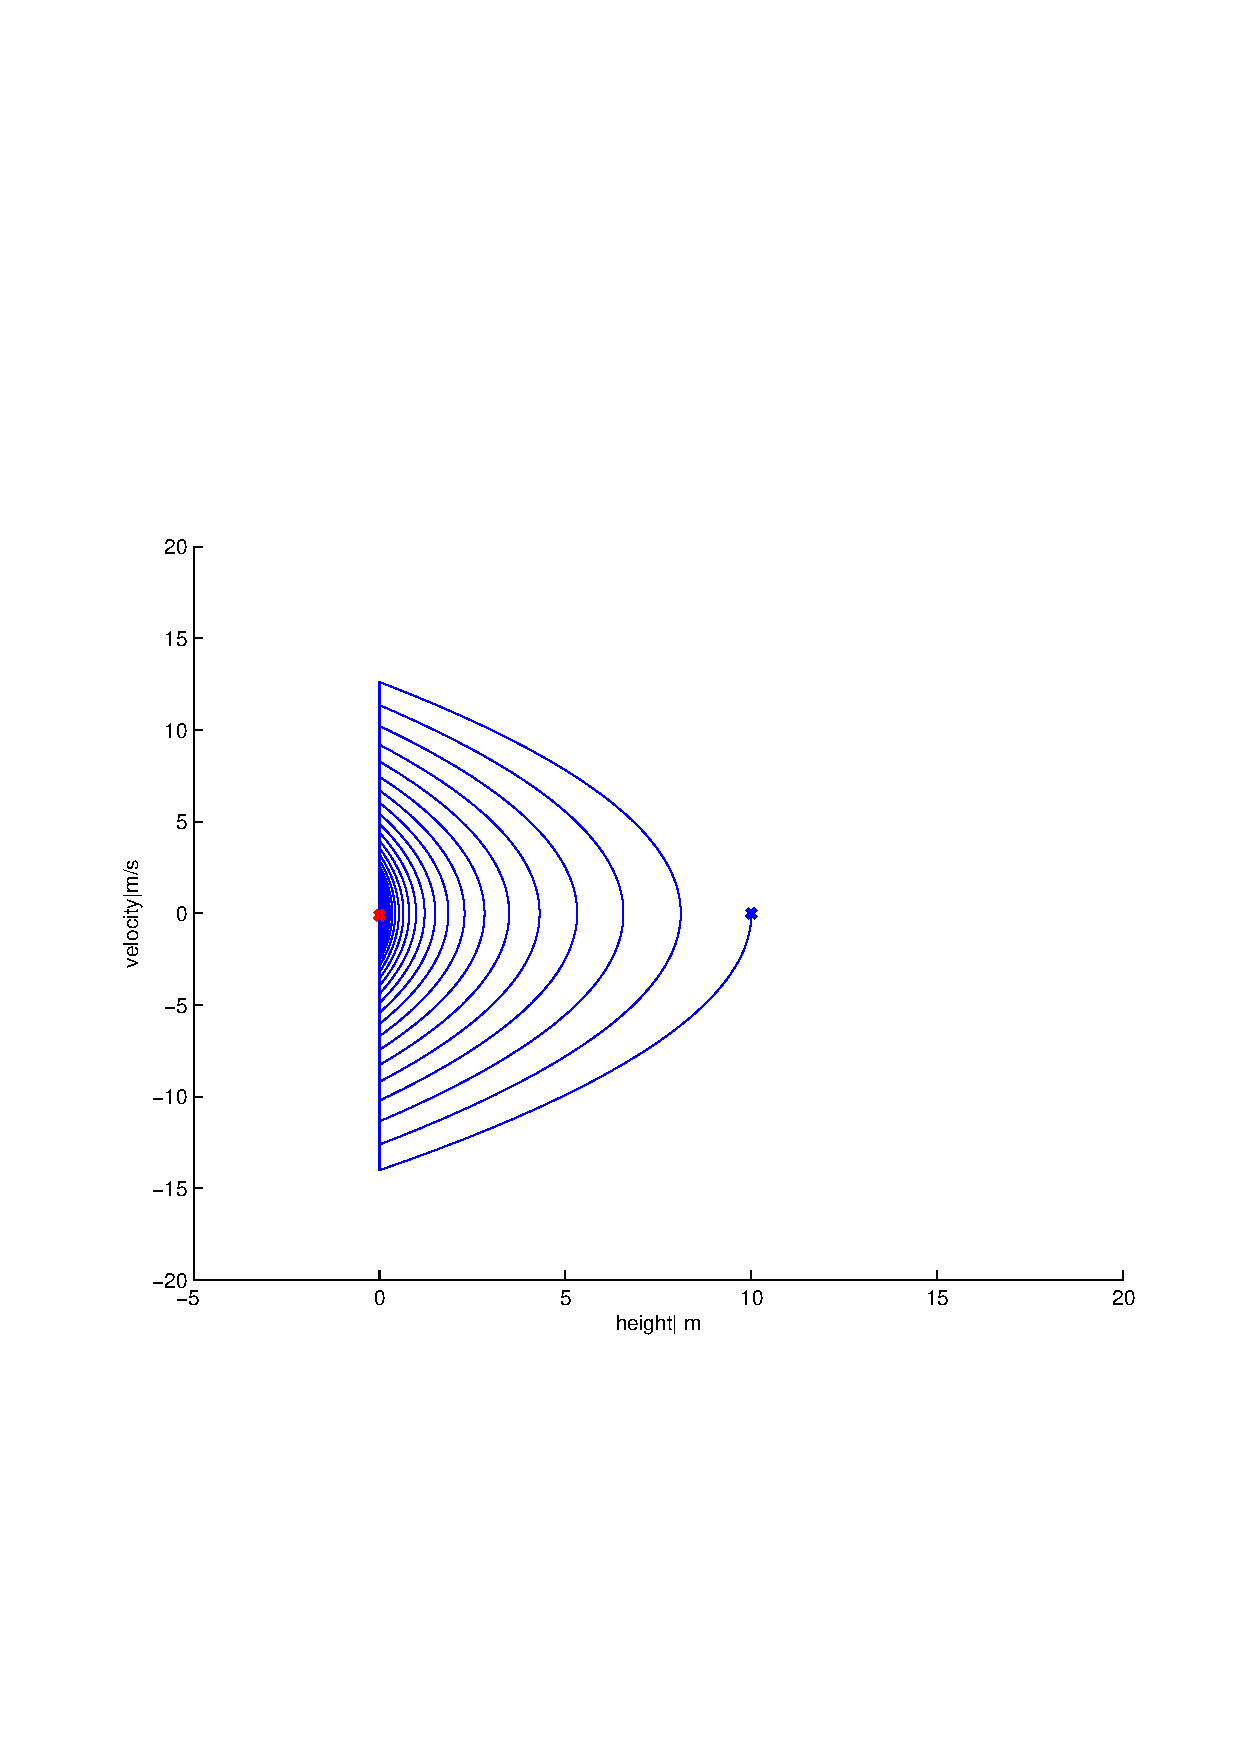
\includegraphics[width=0.7\textwidth]{BouncingBallPhasePlotuncontrolledDropAt10}
    \caption{Drop at 10}
    \label{fig:bouncing10}
\end{center}
\end{figure}

